In this chapter, we revisit the proposed KPIs of the two services, and evaluate them in regards to the framework implementations. As explained in Chapter \ref{ch:methodology}, the KPIs are meant to verify the requirements of the services, so we could confirm the effectiveness of the frameworks. After that, a summary will be made to compare the frameworks in overall.

\section{S1 KPIs evaluation}
In \textbf{S1} (Production Prediction), four KPIs are highlighted (see also Table \ref{tab:s1kpi}), namely, \textbf{level of automation}, \textbf{updating delay}, \textbf{data history}, and \textbf{modifiability}. 

\subsubsection{KPI1: level of automation}
This KPI measures the number of manual steps required in order to support the operations of the framework. Generally, fewer steps are desired as it indicates the framework has a higher level of automation. The steps referred here contribute toward the requirement \textbf{R1}---validate the model states with real-time data.

In practice, the notion of ``step" depends on the architecture of individual frameworks and the use cases. For the purpose of comparison, we have identified four primary actions that occur in \textbf{R1}: data collection, data integration, model scheduling, and status reporting. The manual steps contribute to the automation of these actions in runtime. Note that the actions we have identified here are specific to the microbrewery context. For other use cases, more or fewer actions might be needed to achieve the outcome.

In TwinOps, the collection of monitoring data is handled automatically by Kafka. The openness of the SSP format---which defines the connections between models---allows the internal variables of models to be accessed easily. The core validation process, which includes validating the simulations against real-world data and reporting the new model states, takes place in the CI/CD pipelines. The pipelines are configured in the YAML file by the user ahead of executions. This configuration is the only manual step in the full process cycle. In other words, once the pipelines are pre-configured, the rest of the process should run automatically.

As an IoT-based framework, ThingsBoard uses application-layer protocols that enhance the simplicity in data collection, shielding the user from handling low level communications. However, due to the lack of native model editor supports, the monitoring data and the models are integrated externally to the platform environment during the running of the system. In consequence, a manual step is required for interfacing back to the platform after the integration is complete. Because of that, it poses another disadvantage such that scaling could be hindered as more models are introduced. The model scheduling and its status reporting are automated using \textit{rule chains}. The user is tasked to manually define the \textit{entities} (e.g., sensors) and their \textit{relations} (e.g., sensors are \textit{contained} by the models) before the beginning of \textit{rule chains}. In overall, the two manual steps identified here are interfacing the model editor and entity provisioning. 

Ptolemy II comes with an actor type Accessors that supports external communication. In term of data integration, both the built-in \texttt{FMUImporter} and the \texttt{FMU proxy}---which we opted for---bear resemblance to a blackbox. It means that accessing the internal model states is difficult to achieve unless with an external model editor. Hence, facing the same situation as ThingsBoard, the user has to implement an additional interface. The model scheduling is automatically maintained by the MoC director and the clock actors. As we mentioned earlier, Ptolemy II lacks a data storage feature that suites our DT service. Therefore the user has to establish data logging externally, Kafka has been manually integrated for this task. All things considered, the two manual steps are interfacing the model editor and interfacing the data manager.

Table \ref{tab:kpi1compare} shows a summary of manual steps in each framework. TwinOps is the most automated framework, followed by ThingsBoard and Ptolemy II, as both require some patchworks by the user for different stages of the operation. As we can see, TwinOps enables the user to manage an extensive range of configuration options prior to runtime, it leads to less inconveniences in term of making further patchworks in various parts of the system, as in the cases with the other two frameworks. Additionally, it could also mean less risks for human errors to occur.

\begin{table}[hbt!]
\centering
\begin{tabularx}{\textwidth}{|X|p{3.5cm}|p{3.5cm}|p{3.5cm}|}
\hline
\textbf{} & {TwinOps} & {ThingsBoard} & {Ptolemy II} \\ \hline           
\textbf{Manual steps} & Pipelines configuration & (1) Interfacing model editor. (2) Entity provisioning. & (1) Interfacing model editor. (2) Interfacing data manager. \\ \hline             
\end{tabularx}
\caption{S1 KPI1 comparison}
\label{tab:kpi1compare}
\end{table}

\subsubsection{KPI2: updating delay}
We define updating delay as the time between when the framework has collected all required data and when the updated model states have been computed. Therefore, each updating cycle begins from the completion of data collection and ends in the completion of new model states output. We find that one of the main factors influencing this KPI is the communication style of the orchestration, for instance, whether it relies on external protocols or using in-memory communication. Another factor is due to the initialization process. For cloud based platforms this relates to the initiation of the ``workers" and to their load balancing algorithm, i.e., the allocation of computational power. For platforms that are hosted in local premises, loading the required resources also contributes to delays.

\begin{figure}[hbt!]
  \centering
  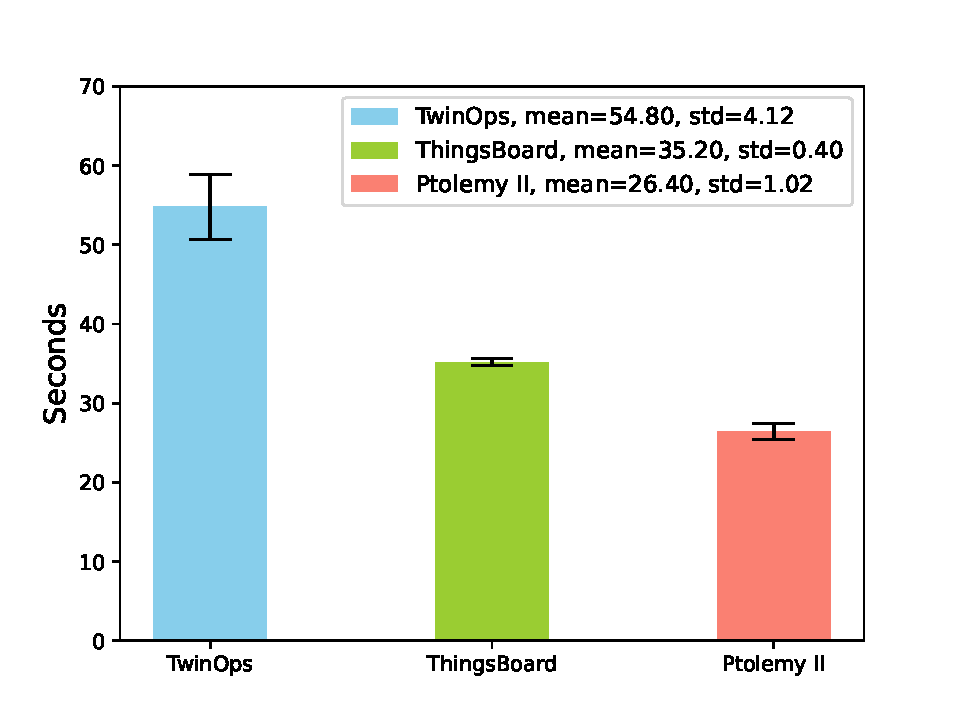
\includegraphics[scale=0.5]{figures/s1kpi2.pdf}
  \caption[S1 KPI2: updating delay]{S1 KPI2: updating delay mean value and standard deviation}
  \label{fig:s1kpi2}
\end{figure}

Figure \ref{fig:s1kpi2} shows the statistics of five updating cycles presented in a bar chart. We observe that TwinOps has the highest mean delay time as well as the greatest standard variation. This is due to the CI/CD engine being hosted in the cloud (as with most popular CI/CD engines in the market), such that it is subject to a user's pricing plan, which results in different load balancing strategies imposed by the cloud server. To keep the measurement consistent, the five updating cycles all use the same free-tier plan.

In ThingsBoard, the orchestration communication utilizes a combination of remote procedure call (RPC) and RESTful protocol. Both are  high level protocols that suggest more packet overhead. This results in the moderate delay time we have seen. In most cases, protocol APIs tend to use buffering techniques to ensure QoS, including mitigation of delay time variance. In ThingsBoard we have already seen that being imposed by the background process as \texttt{TbServiceQueue} in Chapter \ref{ch:implementation}.

For Ptolemy II, given that we use the \texttt{FMU proxy} instead of \texttt{FMUImporter}, a communication overhead is expected. Surprisingly, the mean delay time is the lowest among all the tested frameworks. There are a few hypotheses to this. Firstly, \texttt{FMU proxy} uses UDP interface for communications, which is a low level connectionless protocol. Therefore it is exempted from delays incurred by the excessive handshakes often found in connection-oriented or high level protocols. Secondly, Ptolemy II holds all of its processes together in an unified software package, meaning it needs few external communications or memory fetching beyond the program scope, in contrast to the modular architecture of TwinsOps or ThingsBoard.

It is important to acknowledge a limitation of this KPI measurement, which is that since the frameworks permit quite flexible building block choices for the user, the technologies adopted in the framework may considerably affect the system timing behaviors. For example, one might use a CI/CD engine that is not cloud-based and possibly achieve a much lower delay time; or one could opt for another M2M protocol that is not built-in to ThingsBoard, thus increase or decrease the overall communication latency. The KPI results presented here should be regarded as a reflection of our particular microbrewery DT setup, serving as a reference instead of an absolute judgment.

\subsubsection{KPI3: data history}
Data history concerns the amount of historical data ready to be used for the service. For context, the data are being used for computing future heat transfer in \textbf{S1}.

In TwinsOp, the user is able to add steps inside the CI pipeline that archive data as artifacts. On the other hand, in the CD pipeline, as we have discussed, data are containerized as images and stored in the online repository. ThingsBoard framework provides native data storage that is integrated with the \textit{rule engine}, such that the historical model states and events are constantly recorded in background. Ptolemy II on its own lacks an efficient data management system. However, we manage to solve that shortcoming by integrating the Kafka service.

In overall, all three frameworks are able to retain all historical data for the full lifecycle of the service.

\subsubsection{KPI4: modifiablility}
This KPI concerns two main aspects: the configuration of model initial values; and the configuration workflow of model executions. Our use case reveals that each framework offers varying degrees of configurability before and after startup, as discussed below.

Due to the modular nature of TwinOps, a user can customize all stages of the framework workflow, including the control of the model executions. In terms of initial value setting for the models, it could be accomplished in the SSP file. Table \ref{tab:twopconfig} summarizes the initial configuration options accessible by the user. Once all the configuration options are settled, the DT should be able to operate automatically.

\begin{table}[hbt!]
\centering
\begin{tabularx}{\textwidth}{|p{1.5cm}|p{3.5cm}|p{3.5cm}|X|}
\hline
\textbf{Type} & {SSP} & {YAML} & {Dockerfile} \\ \hline           
\textbf{Format} & \texttt{.ssp} & \texttt{.yml} & No file extension  \\ \hline
\textbf{Scope} & models editor & CI/CD engine & CI/CD engine \& container repository \\ \hline
\textbf{Purpose} & Define the execution flow and data dependencies between FMUs & Validate the updated model states & Deploy to the target platforms \\ \hline    
\end{tabularx}
\caption{TwinOps initial configurations overview}
\label{tab:twopconfig}
\end{table}

Likewise to TwinOps, the ThingsBoard framework is also highly customizable, such that all workflow stages can be configured at the beginning. Furthermore, the \textit{entity management} provides the option to set initial values and attributes to the model entities. The summary of configuration options is shown in Table \ref{tab:tbconfig}.

\begin{table}[hbt!]
\centering
\begin{tabularx}{\textwidth}{|p{1.5cm}|p{3.5cm}|p{3.5cm}|X|}
\hline
\textbf{Type} & {CSV} & {JSON} & {Configuration} \\ \hline           
\textbf{Format} & \texttt{.csv} & \texttt{.json} & \texttt{.conf}  \\ \hline
\textbf{Scope} & Entity management & Profile \& rule chain \& dashboard & ThingsBoard backend services\\ \hline
\textbf{Purpose} & Provision entities and define their relations & Setup device profiles, rule chains, and dashboards & Set parameters to ThingsBoard background processes such as memory allocation, timeout, etc.\\ \hline    
\end{tabularx}
\caption{ThingsBoard initial configurations overview}
\label{tab:tbconfig}
\end{table}
 
In contrast, the architecture of the Ptolemy II workflow is relatively monolithic and closed compared to the other two frameworks. Designing is done in the GUI of the software, where the operator performs drag-and-drop on the icons representing directors and actors, though there is the option to import or export the design in XML format. The operator could alter the execution flow by choosing the MoCs, represented by directors. Although the MoCs account for the timing progression of models, they do not address the configurations for the data collection before the model update and the data storage after the model update. It suggests the modifiablility of Ptolemy II is inadequate to cover the entire workflow for the service. Many actors in Ptolemy II do not support initialization of model parameters. Therefore, a workaround has to be made by using input variables. Although it does not affect the functionality, potential confusions may arise for the downstream user who does not develop the models in first hand.

\section{S2 KPIs evaluation}
In \textbf{S2} (Production Control), two KPIs (see also Table \ref{tab:s2kpi}) will be evaluated, which are \textbf{traceability} and \textbf{latency}. 
\subsubsection{KPI1: traceability}
In context, the traceability is concerning how much information is available to the operator which they can use to evaluate the effects of the DT's controlling actions.

In TwinOps, the building blocks in each workflow stage are only loosely coupled, they are each an independently deployable module. As a result, the trace of a model's behaviors can be quite scattered. When progressing through stages, the model artifacts, such as connection links, parameters, and states, tend to undergo format transformations that will lose some explicitness of the traces.
To illustrate, the models topology is visualized in the model editor stage, but in the CI/CD stage it becomes a part of pipeline instructions that is no longer easily readable by humans. From the CI/CD stage to the containerizing stage, another transformation occurs as the pipeline instructions are brought into a container image which requires another service (e.g. docker) to run. To sum up, the consistency of trace explicitness is often lost during the transfer of data ownership from one stage to another.

As we have seen in the dashboard demonstration in Section \ref{sec:s2demo}, the ThingsBoard framework handles the system traceability very well. It is attributed to the highly integrated operability between the \textit{rule engine}, the data storage, and the real-time dashboard. When data ownership is transferred between them, the framework ensures the data properties, e.g., timestamps, data types, etc, remain consistent throughout. Therefore, one is able to easily trace an effect back to its root cause.

In theory, Ptolemy II supports the transfer of data ownership, meaning an actor will gain full controls of data once receiving from another actor. However, this is more true when two actor types are alike. When the types are significantly different, such as between a server actor---which sends and receives internet packets---and a mathematical operation actor, all kinds of errors may occur. The user has to make sure the conversion is done properly. As more kinds of actors are adopted to support the growing DT service, it becomes harder to scale up this kind of pairing conversion. Eventually making the system traces harder to track.

\subsubsection{KPI2: latency}
This KPI measures the latency between the finishing of model updates and the completion of the control triggering. It indicates the responsiveness of the framework in dealing with VE-PE communications. Figure \ref{fig:s2kpi2} shows the statistics of five measurements.

It can be seen that TwinOps has the highest mean and standard variation. It is again due to the load balancing mechanism managed by the CI/CD host server. ThingsBoard and Ptolemy II have similar mean latency, but the former clearly has the lower of the two variances.

This KPI suffers the same limitation as \textbf{S1 KPI2}. The timeliness is sensitive to the high variability of technology choices made by the user. Although we can see a general pattern here that a centralized system such as Ptolemy II has lower latency than distributed systems like TwinOps.

Aiming for low mean latency and low variance are two particularly important properties for a time critical system, even though the microbrewery DT is not one such system. They affect the bound for worst case execution time (WCET), which is a determining factor in schedulability analysis, i.e., the computation deciding whether a set of tasks are able to meet the deadline in a real-time system.

\begin{figure}[hbt!]
  \centering
  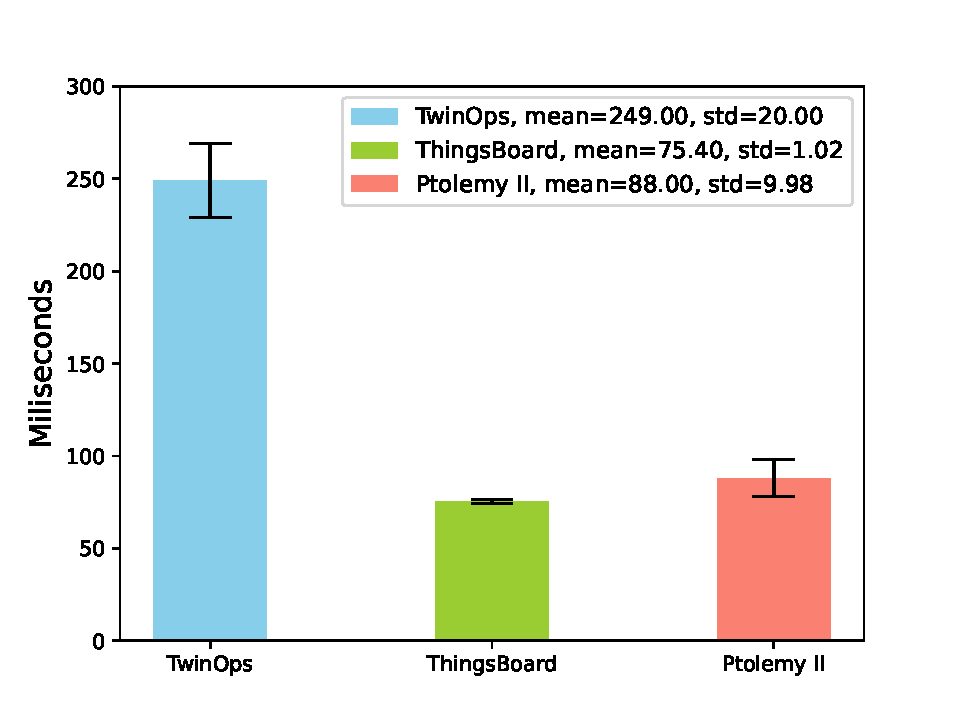
\includegraphics[scale=0.5]{figures/s2kpi2.pdf}
  \caption[S2 KPI2: latency]{S2 KPI2: latency mean value and standard deviation}
  \label{fig:s2kpi2}
\end{figure}

\section{Summary of framework comparison}
This section summarizes the most significant findings about the frameworks in terms of integration and orchestration. Table \ref{tab:framecompare} shows a side-by-side comparison. The rows represent the categories generalized from the KPIs and the requirements to a broader scope; the columns list the three frameworks. Most categories below have been introduced in the earlier chapters. ``Data transformation" covers the ability to transform the data to other forms or formats for the subsequent stages within the workflow, or for storing in case of future usages. ``Traceability", as explained in the earlier section, is an aspect of data ownership. We have decided to compare the traceability instead of the greater scope (ownership), as it is a narrower---more focused---aspect, making it easier to compare between the considerably different framework styles in this project.
 
\begin{table}[hbt!]
\centering
\begin{tabularx}{\textwidth}{|X|p{3cm}|p{3cm}|p{3cm}|}
\hline
 & \textbf{TwinOps} & \textbf{ThingsBoard} &  \textbf{Ptolemy II}\\ \hline    
\multicolumn{1}{|l|}{\textbf{Integration}} & \multicolumn{3}{c|}{}\\ \hline           
{Configurability} & high & high & medium \\ \hline
{Data transformation} & high & medium & medium \\ \hline
{Traceability} & complex & simple &  simple (but inefficient) \\ \hline
{Modularity} & high & medium & low \\ \hline   
\multicolumn{1}{|l|}{\textbf{Orchestration}} & \multicolumn{3}{c|}{}\\ \hline  
{Workflow automation} & high & medium & low\\ \hline
{Timeliness} & slow & fast & fast\\ \hline
{Managing diversity} & good & good & good (but requires external add-ons) \\ \hline 
\end{tabularx}
\caption{Framework comparison}
\label{tab:framecompare}
\end{table} 
 
Regarding the integration aspects, TwinOps is highly configurable and modular, credited to its multi-stage architecture; its data can be transformed effectively to adapt to different stages of the workflow. However, the same features make it difficult to conduct explicit ownership transfer of model artifacts, meaning the methods for data accessing may vary considerably in different stages. This can hinder the traceability of the DT behaviors. ThingsBoard also has high configurability. The components within the framework are more cohesive, resulting in a more consistent data ownership and medium modular potential. Ptolemy II, being a self-contained software, has limited---under the DT context---configuration options and limited modularity. Some data transformation can be performed by the actors, although it is often not necessary as the processes in the workflow are already tightly coupled. The actor-orientated architecture is conducive to a consistent data ownership although extra patches, such as data format conversions from one actor type to another, are often needed. That makes the tracing of the system become inefficient.

For the orchestration aspects, TwinOps is able to attain the highest automation; we argue it is correlating to the extensive preliminary configurations. It is quite slow, because the cloud-based CI/CD engine focuses on the ``continuity" angle instead of the ``speed" angle of operation. ThingsBoard takes advantages of its IoT networking backends, resulting in decent automation and decent speed. For Ptolemy II, the workflow requires some manual implementations from the user to automate. It is fast since the framework is relatively more centralized, thus its components suffer less from communications and synchronizations penalty.

Finally, all three frameworks manage to satisfy all requirements of the DT services, even though their KPIs show the weaknesses and caveats that the user has to keep in mind of during the development process. The frameworks are capable of managing diverse types of entities in the microbrewery DT, presuming the requirement for time criticality is not strict, as is the case with fermentation processes.